\newcommand{\bs}{\mathbf{s}}
%------------------------------------------------------
\begin{figure*}[!t]
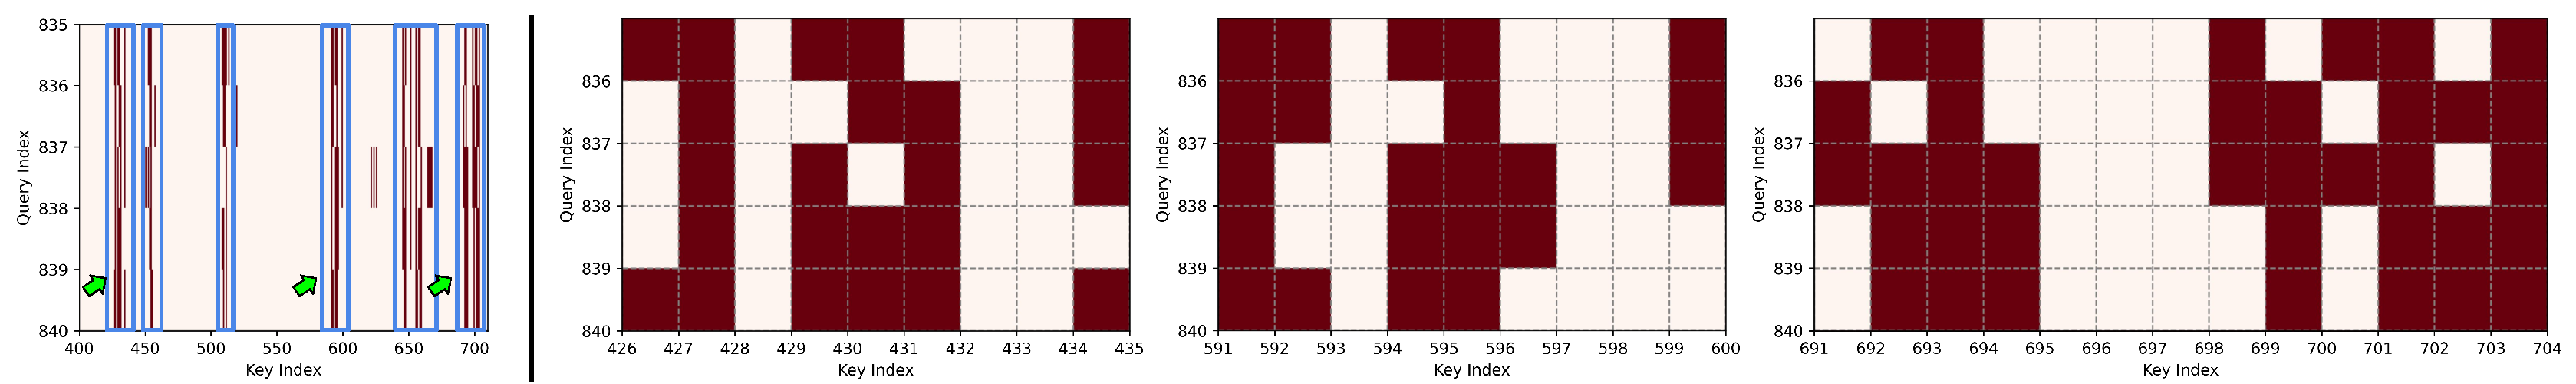
\includegraphics[width=1\textwidth]{assets/attn-cluster.pdf}
\centering
%\vspace{-0.5em}
    \caption{\textbf{Distribution of critical indices in LLaMA2-7B-Chat (Layer 10, Head 2).} For each query, we retrieve 64 critical indices using the top-$k$ oracle on WikiText2. Columns show five temporally adjacent queries with cosine similarity $>\!0.8$. \emph{Left}: overall distribution across keys 400–710; clusters are outlined in \textcolor{blue}{blue boxes}. \emph{Right}: zoom-ins of three clusters (annotated by \textcolor{green}{green arrows} in the left) at keys 426–436, 591–700, and 691–704. Critical indices are in \textcolor{red}{red}.}
    \label{fig:attn-cluster}
    \vspace{-0.5em}
\end{figure*}
%------------------------------------------------------

%  from the same layer–head


%\vspace{-0.05in}
\section{Observations and Properties}
%\vspace{-0.05in}
\label{sec:observations}

While empirical priors (temporal locality, recency, cross-layer redundancy) are suggestive, PrHS requires \emph{query-independent} design rules that can be applied pre-hoc without full attention. Accordingly, from the transformer’s mechanics we derive two properties: (i) clustered locality and among-query continuity of critical indices, and (ii) progressive cross-layer propagation of information. These properties motivate our selector parameterization and, in Sec~\ref{sec:method}, yield a retained-mass guarantee $\tau_{\mathrm{pre}}\!\ge\!\tau^*-\beta_{\mathrm{th}}$, which translates to MI bounds via Eq.~\eqref{eq:mi_bound}.


%------------------------------------------------------
\begin{figure}[!t]
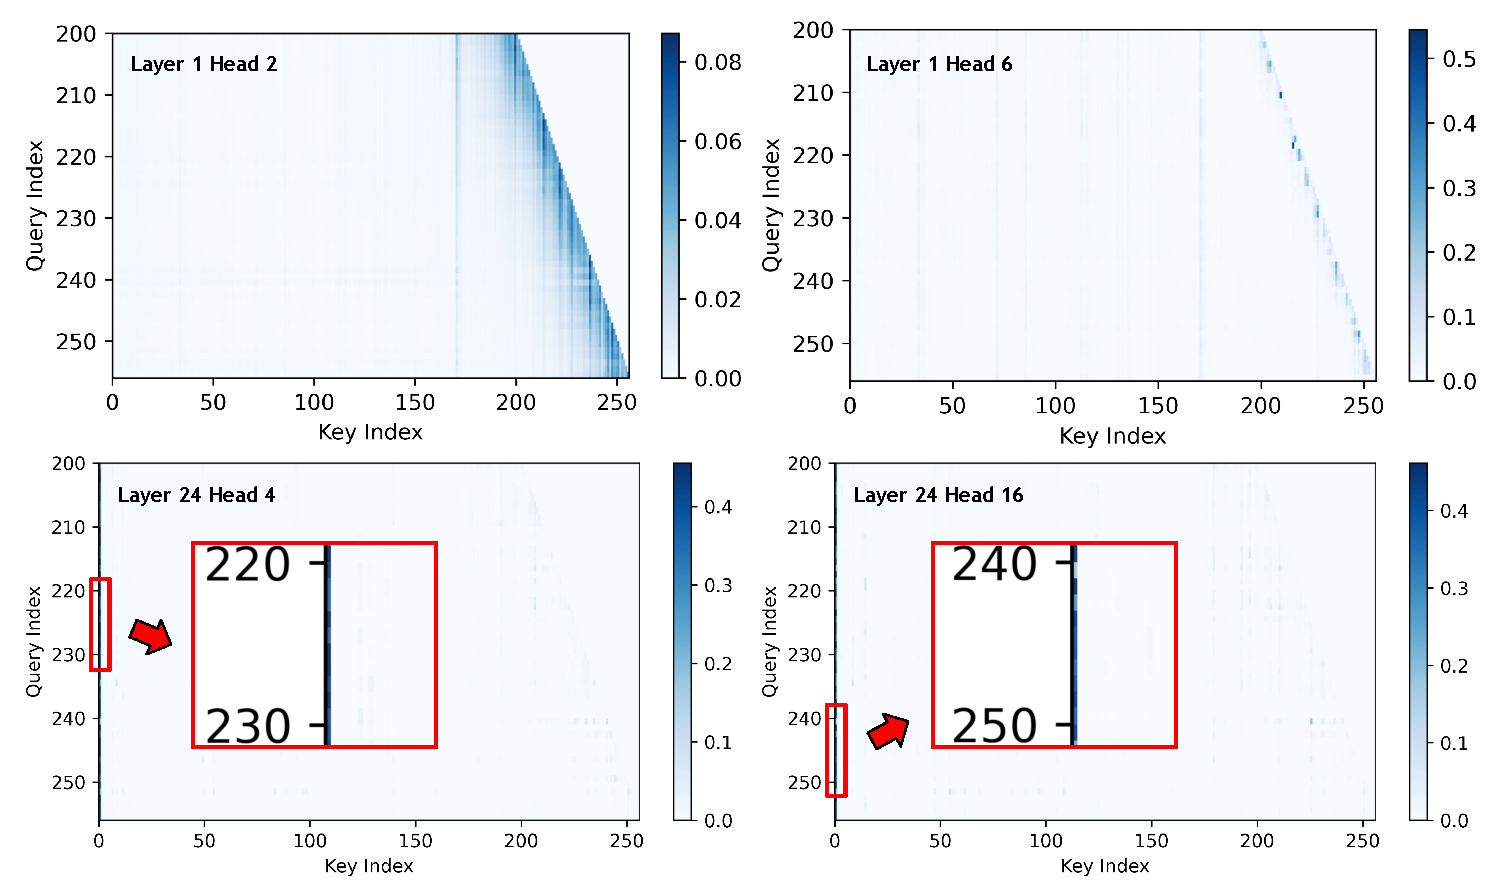
\includegraphics[width=0.45\textwidth]{assets/attn-distribution.pdf}
\centering
\vspace{-0.5em}
    \caption{\textbf{Attention distribution on LLaMA2-7B-Chat.} Heatmaps across representative layer–head pairs, with darker color indicating stronger attention.}
    \label{fig:attn_dis}
    \vspace{-1em}
\end{figure}
%--------

\subsection{Observation 1: Critical Tokens Exist in Clustered Manners}

Prior work~\cite{sun2024shadowkv,li2024snapkv,wuhshare} shows that consecutive decoding queries are close in embedding space and often share critical indices, which motivates KV sharing strategies. However, \emph{per-head} selections can still vary markedly, and the overlap between selected indices remains small even for high cosine similarity between queries~\cite{wu2024tokenselect}, leading to
suboptimal sharing. For example, HShare~\cite{wuhshare} shares indices directly, missing many truly critical indices at high sharing ratios.
To bridge this gap, we observe that critical indices organize into a small number of clusters that persist across adjacent queries, providing a more stable sharing
unit than individual indices. 

\begin{property}[Among-query Property]
\label{prop:among-query}
For two semantically similar consecutive queries, the centroids of their critical-token clusters undergo a smooth mean shift along the sequence axis.
\end{property}

As shown in Fig.~\ref{fig:attn-cluster}, when the cosine similarity between $q_t$ and $q_{t+1}$ exceeds $0.8$, critical indices concentrate into a few clusters; although cluster centers and spreads shift slightly, the cluster-level overlap remains large. Our theoretical analysis further shows that these clusters satisfy a mean-shift (bounded drift) property, formalized in \textbf{Theorem}~\ref{the:mean-shift}.

\begin{theorem}[Centroid Drift]
\label{the:mean-shift}
Consider the scaled dot-product self-attention (cf. Eq.~\eqref{eq:attn_eq}) with fixed keys $\{\bk_j\}_{j=1}^t$, attention weights $A_j(\bq_t)$ for key $\bk_j$, and let $\{p_j\}_{j=1}^t$ be scalar token positions with
$\mathrm{diam}\,\mathcal{P}:=\max_j p_j-\min_j p_j$ for $\mathcal{P}=\{p_j\}$. Define the sequence-axis centroid $c(\bq_t)=\sum_{j} A_j(\bq_t)\,p_j$. For $\bq' = \bq_t + \Delta$ with $\|\Delta\|\ll 1$,
\begin{equation}
\label{eq:centroid_shift}
    c(\bq') = c(\bq_t) + O(\|\Delta\|),
\end{equation}
\textit{i.e., the attention centroid moves in a Lipschitz-continuous fashion with respect to the query. In particular, $|c(\bq')-c(\bq_t)| \le (\mathrm{diam}\,\mathcal{P})\,\frac{\max_j \|\bk_j\|}{\sqrt d}\,\|\Delta\|$.}
\end{theorem}
The drift is $\mathcal{O}(\|\Delta\|)$ with Lipschitz modulus
$L \le (\mathrm{diam}\,\mathcal{P})\,\max_j \|\mathbf{k}_j\|/\sqrt{d}$.
This smooth drift is consistent with empirical attention patterns and with
StreamingLLM’s “keep a few initial tokens” observation~\cite{xiao2023streamingllm}.


In summary, \textbf{across heads and layers, the critical tokens of successive similar queries form dense, localized clusters}. We call this the \textbf{sink effect}: \textit{tokens near a high-attention location inherit elevated attention due to semantic proximity}. Exploring the effect enables explicit control under PrHS, our CIS operationalizes this by dilating shared sets to cover the local cluster and compensate for centroid drift, avoiding full per-head re-retrieval. Detailed proofs are in \textbf{Appendix A}.



\subsection{Observation 2: Information Propagates Progressively Among Layers}

Locality-bias analyses~\cite{zhang2023h2o,ge2023fastgen} show that attention is
sharply concentrated locally within a narrow window around the current query
and the sink token, across diverse prompts (Fig.~\ref{fig:attn_dis}).
This suggests that the current token draws most information from recent tokens,
whereas the sink token acts as an attractor rather than conveying semantic content.
Viewed in isolation, such constrained receptive fields would only support short-term memory for LLMs, seemingly at odds with their strong long-context performance.
Moreover, recent studies~\cite{cai2024pyramidkv,wan2024d2o,gao2023empower} show that:
across layers, intermediate tokens incrementally absorb the semantics of their relevant predecessors; by higher layers, a mid-sequence token encodes both its own content and a compressed synopsis of earlier, distant tokens.
It means that stacking transformer layers realizes long-range dependency paths through chains of neighboring tokens even when no individual layer attends broadly.
Consequently, salient long-distance information is distilled into nearby carrier
tokens, reducing the marginal importance of many earlier ones; hence,
later layers need not re-scan the full prefix.
Building on this insight, PSAW and ETF prune KV entries whose instantaneous (per-layer) and accumulated (cross-layer) attention mass fall below preset thresholds, ensuring that the total dropped mass remains within $\beta_{\mathrm{th}}$; by Eq.~\eqref{eq:mi_bound}, this certifies a bounded MI loss.
We formalize these guarantees in \textbf{Appendix C-D}.


% Prior work~\cite{sun2024shadowkv,li2024snapkv,wuhshare} shows that adjacent queries are close in embedding space and share many critical indices, motivating KV sharing techniques. However, \emph{per-head} selection among these queries can still differ markedly, and overlap remains small even when queries are nearly identical~\cite{wu2024tokenselect}, yielding suboptimal KV sharing results. For example, HShare~\cite{wuhshare} shares indices directly, missing many truly critical indices at high sharing ratios. To close this gap, we observe that critical indices form \emph{clusters} that persist across adjacent queries, and formalize this in Property~\ref{prop:among-query}.

%Locality-bias analyses \cite{zhang2023h2o,ge2023fastgen} show that, attention is sharply local-concentrated within a narrow window around the query plus the sink token, regardless of prompts, as shown in Fig.~\ref{fig:attn_dis}. This indicates that the current token absorbs most of information from recent tokens, as sink token is a placeholder and does not convey any actual content. Viewed in isolation, such constrained receptive fields would only support short-term memory for LLMs, seemingly at odds with their strong long-context performance. While recent studies~\cite{cai2024pyramidkv,wan2024d2o,gao2023empower} show that: across layers, intermediate tokens incrementally absorb the semantics of its relevant predecessors; by higher layers, a mid-sequence token encodes both its own content and a compressed synopsis of earlier, distant tokens. Thus, stacking transformer layers realizes long-range dependency paths through chains of neighboring tokens, even when no individual layer attends broadly. As such, salient long-distance information is distilled into nearby carrier tokens, reducing the marginal importance of many earlier ones. Therefore, \textit{later layers need not re-scan the full prefix}. PSAW and ETF prune KV entries whose instantaneous (per-layer) and accumulated (cross-layer) attention mass fall below preset thresholds, so that the total dropped mass stays within $\beta_{\mathrm{th}}$, following the bounded MI loss in Eq.~\eqref{eq:mi_bound}. We formalize these guarantees (Theorem~\ref{the:error_bound}) once PSAW and ETF are in place.
